\paragraph{Pre-registered held-out replication.} We committed a replication script before running it (\texttt{gnomad\_replication}): 30 CLIP miRNAs outside the discovery panel, a one-sided test in the discovered direction, and a new UTR-length-matched control (decile matching on the longest 3$'$ UTR). Gates passed (97.8\% coverage). The reversal replicates: the CNN top-200 is less constrained than uniform random in 30/30 miRNAs ($p=9.3\times10^{-10}$; median LOEUF difference +0.192), than expression-matched sets in 30/30 ($p=9.3\times10^{-10}$; +0.161), and than UTR-length-matched sets in 25/30 ($p=1.6\times10^{-4}$; +0.084; Figure~\ref{fig:gnomadrep}). CNN top-200 genes have shorter UTRs than their universe in 30/30 miRNAs, and length matching shrinks the gap, but it does not remove it.
At that point we treated this as a falsifiable candidate pattern, not a confirmed mechanism. Subsequent pre-registered dosage-label tests (DECIPHER, ClinGen, HPO) did not support the clause about UTR length, so we withdrew it (Table~\ref{tab:decipher}). The later locked random-weight falsifier also failed: untrained weights reproduce the apparent depletion at the required panel-count threshold. We therefore withdraw the learned-model biological claim entirely, despite this descriptive held-out-gene pattern. A finer absolute UTR-length-bin audit, run after the failed falsifier, is reported separately below; it cannot restore the failed gate. Purifying selection was only an untested hypothesis, not an inference here.
\begin{figure}[h]\centering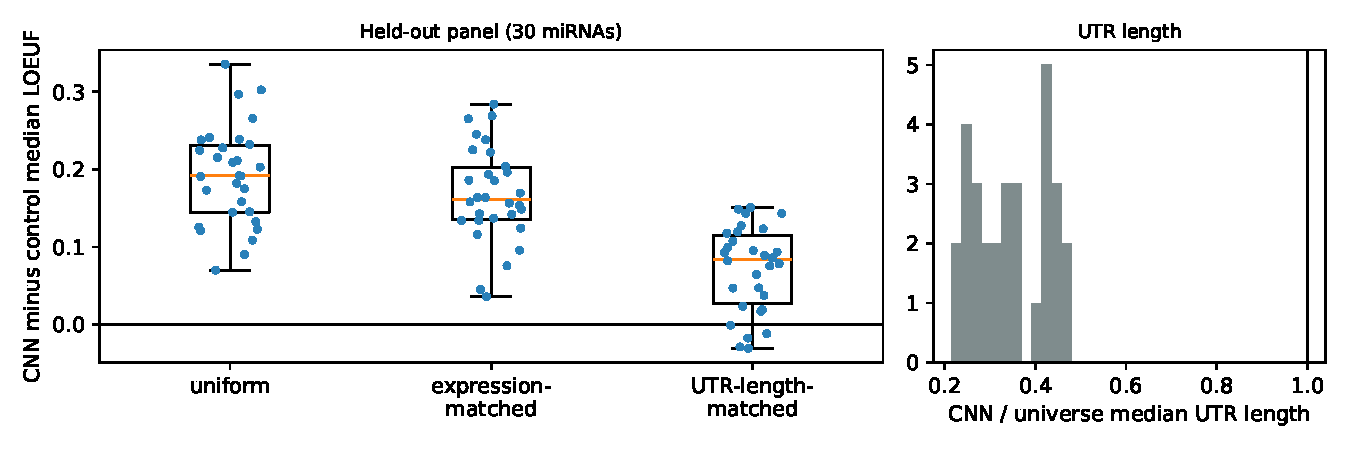
\includegraphics[width=0.95\linewidth]{figs/fig_gnomad_rep.pdf}
\caption{Pre-registered replication on 30 held-out miRNAs. Left: CNN top-200 median LOEUF minus each control (positive = CNN less constrained). Right: CNN top-200 median UTR length relative to its universe.}\label{fig:gnomadrep}\end{figure}
